% Anforderung
\chapter{Funktionale Anforderungen}
\label{sec:anforderung}
% Text

Um eine solide Grundlage für die Entwicklung einer Anwendung zu haben, benötigt es ein Lastenheft, das vor dem Entwicklungsprozess definiert werden muss. Die oberste Priorität in einem solchen Lastenheft haben die Anforderungen des eigentlichen Auftraggebers. Zusätzlich wurden nach Wunsch des Auftraggebers noch weitere Anforderungen aus dem International Office und dem Sprachenzentrum gesammelt. Diese zwei Teile des Lastenhefts richten sich nach einer der Säulen des Leitbilds der Hochschule Hof, der Internationalisierung mit Fokus auf Indien. Im folgenden werden die gesammelten Anforderungen an die web-basierte Hochschul-\ac{App} genauer betrachtet.

\section{Auftraggeber\label{sec:anforderungen_ag}}

In den vergangenen Jahren wurden die Anwendungen der Hochschule Hof durch verschiedene Professoren und Mitarbeiter der Hochschule Hof beaufsichtigt und geleitet. Im vergangenen Sommersemester 2019 ist die Zuständigkeit der Android \ac{App} an Prof. Dr. Heym übergegangen. Statt sich jedoch auf die plattformabhängige Version zu fixieren strebt dieser es stattdessen an, eine betriebssystemunabhängige Anwendung zu schaffen, die auf allen Endgeräten funktioniert und dennoch für mobile Endgeräte optimiert ist.

\subsection{Grundlegende Anforderung}
%urspr. Allgemeines

Der Fokus soll in der kommenden \ac{App} darauf liegen, dass sie für alle Anwender gleich nutzbar ist, unabhängig davon, welches Endgerät genutzt wird, ob \ac{PC}, Smartphone oder Tablet. Auch das Betriebssystem soll dabei keine Rolle mehr spielen. Zudem ist ein großer Beweggrund für diese Arbeit die Neuentwicklung einer Anwendung, welche durch die gesammelten Erfahrungen der \acp{App} der vergangenen Jahre an die Bedürfnisse der Nutzer angepasst wird.  

\subsection{Funktionale Anforderungen}

Im folgenden werden die Anforderungen und deren Gewichtungen aufgeführt und näher erläutert.

\subsubsection{Stundenplan}

Wie in allen Anwendungen der Hochschule Hof ist die zentrale Funktion der \ac{App} das Anzeigen des Stundenplans. Dieser Stundenplan soll sich allgemein nach dem Studiengang und dem Fachsemester des Anwenders richten. Zusätzlich soll es einen personalisierten Stundenplan geben, den sich der Nutzer eigenständig zusammenstellen kann. Anders als in den bereits vorhandenen Anwendungen soll der Fokus des Stundenplans auf der Personalisierung liegen. 
\\
\linebreak
Hierbei soll auf folgende Punkte geachtet werden:

\begin{itemize}
	\item Fakultät des Nutzers
	\item Studiengang des Nutzers
	\item Fachsemester des Nutzers
	\item Einfache Einbindung nicht regulärer Vorlesungen
	\item Einfache Einbindung des erweiterten Vorlesungsspektrums der Hochschule (z.B. Sprachkurse)
\end{itemize}

\subsubsection{Stundenplan Änderungen}

Zusätzlich zu den allgemeinen Stundenplan Informationen und der personalisierten Ansicht sollen auch die Änderungen im Vorlesungsprogramm dargestellt werden. Hierbei ist zwischen langfristigen Änderungen und den einmaligen Änderungen zu unterscheiden. Langfristige Änderungen könnten zum Beispiel dauerhafte Raumänderungen, Wechsel des Dozenten oder die Absage einer Veranstaltung sein. Diese sollten automatisiert angepasst werden, wobei dem Nutzer einmalig mitgeteilt werden soll, dass sich diese Veranstaltung geändert hat. Kurzfristige Änderungen hingegen sind Änderungen, welche Einmalig eintreten. Darunter fallen zum Beispiel einmalige Raumänderungen, Ausfälle durch Verhinderung des Dozenten oder Verschiebungen von Vorlesungen. Diese sollten möglich klar in die Ansicht des Stundenplans fallen, sodass der Nutzer sofort erkennt, dass der aktuelle Zeitplan vom Regelfall abweicht. Zusätzlich soll der Anwender benachrichtigt werden, wenn sich eine Änderung ergibt.

\subsubsection{Speiseplan}

Wie auch in den Anwendungen für Android und Windows soll die neue \ac{App} die Speiseplan Informationen des Studentenwerk Oberfrankens anzeigen. Diese Informationen sollen nach den Wünschen des Anwenders gefiltert werden. Demnach kann sich der Anwender alle Preiskategorien anzeigen lassen oder eben nur die Kategorie, in die er selber auch fällt. Zudem soll standardmäßig das ganze Menü angezeigt werden. Stattdessen soll der Nutzer auch einige Teile des Menüs ausblenden können. So kann ein vegetarischer Nutzer zum Beispiel nur die vegetarischen Gerichte anfordern. Weiterhin sollen die Speisen mit allen zusätzlichen Informationen angezeigt werden, wie zum Beispiel den Inhaltsstoffen und Allergenen.

\subsubsection{Anwenderverwaltung}

Um die weiter oben erwähnten personalisierten Darstellungen der Stundenplan und Speiseplan Informationen anbieten zu können, ohne dass sie bei jeder Öffnung der Anwendung neu eingestellt werden müssen, ist es notwendig, dass eine Anwenderverwaltung implementiert wird. Diese kann dann die nötigen Einstellungen der Nutzer speichern. Diese Anwenderverwaltung soll jedoch so flexibel wie möglich bleiben. Im Fokus stehen nach wie vor die Studierenden der Hochschule Hof, die eine E-Mail-Adresse der Hochschule besitzen. Jedoch ist dies nicht immer der Fall. Die Nutzergruppe der Anwendung kann folgende Studierende enthalten:

\begin{itemize}

\item Reguläre Studierende

\item Gaststudierende

\item Sprachkurs Teilnehmer

\item Internationale Studierende

\end{itemize}

Gaststudierende und Teilnehmer der Sprachkurse sind nicht immatrikuliert und haben demnach auch keine E-Mail-Adresse der Hochschule Hof. Dennoch belegen sie Kurse und sollen einen personalisierten Stundenplan erstellen können. Deshalb ist es wichtig, dass auch sie im Bereich der Anwenderverwaltung berücksichtigt werden. 
\\
\linebreak
Um nicht unnötig Daten zu sammeln und die Nutzer, die nicht mehr an der Hochschule studieren aus der Anwenderverwaltung zu entfernen ist es auch wichtig, dass Nutzerdaten automatisiert gelöscht werden, wenn sie nicht mehr benötigt werden oder der zugehörige Nutzer nicht mehr berechtigt ist, sich anzumelden. Diese Anforderung wird jedoch im Laufe dieser Arbeit nicht weiter betrachtet. Stattdessen wird auf die parallel dazu erstellte Bachelorarbeit zur Authentifizierung und Personalisierung verwiesen\autocite[][]{andreasba}.

\subsubsection{Mehrsprachigkeit}

Neben dem International Office stellt auch der Auftraggeber die Anforderung, die Daten der Anwendung in mehreren Sprachen bereitzustellen. Unter diesen Sprachen sollte demnach mindestens Deutsch und Englisch sein. Das Ziel dieser Anforderung ist es, die Internationalen Studierenden besser zu unterstützen.

\subsubsection{Mobile First}

Wie bereits erwähnt wurde, soll die Anwendung Plattform unabhängig sein. Demnach muss es egal sein, welches Endgerät der Anwender nutzt, um die \ac{App} aufzurufen. Ebenfalls egal ist das Betriebssystem, das auf dem Endgerät installiert ist. Jedoch soll die Anwendung, auch wenn sie sich auf allen Endgeräten gleich verhalten muss, auf mobile Endgeräte angepasst sein. Das bedeutet, dass die Informationsdarstellung und die Navigation primär auf mobilen Endgeräten einfach zu bedienen sein muss. Weiterer Implementierungsaufwand kann dann nach Bedarf noch in die 
dynamische Anpassung an den Client investiert werden.

\section{International Office\label{sec:anforderungen_io}}

Die Hochschule Hof hat sich im Laufe der vergangenen Jahre immer mehr mit dem Thema Internationalisierung auseinandergesetzt. Aus diesem Grund wurde die Internationalisierung mit Fokus auf Indien im Frühjahr 2011 sogar als zentrale Säule in das Leitbilds der Hochschule Hof aufgenommen\autocite[Vgl.][]{campuls}.
\\
\linebreak
Konkret heißt es im Leitbild der systemakkreditierten Hochschule Hof\autocite[Vgl.][]{fhhofwebsite}:
\begin{quote}
Der Erfolg der Absolventen in nachhaltig wirtschaftenden und international agierenden Unternehmen bestimmt das Handeln aller Mitglieder des wissenschaftlichen Unternehmens Hochschule Hof. Die Studierenden werden in unserer  weltoffenen Green Tech University exzellent betreut. Praxisorientierte, international ausgerichtete und der Ressourceneffizienz verpflichtete Aus- und Weiterbildung prägt unsere Arbeit. Die angewandte Forschung sichert die Aktualisierung des Wissens für die Lehre und entwickelt Lösungen zum Nutzen für die Wirtschaft.
\end{quote}
Klar zu erkennen ist hier die mehrmalige Erwähnung der Internationalisierung der Hochschule Hof. Aus diesem Grund wird im Laufe der Neuentwicklung einer Hoch\-schul-\ac{App} auch mit dem International Office der Hochschule Hof zusammengearbeitet.

\subsection{Problem}

Wie bereits im Kapitel \ref{umfrage_zielgruppen} beschrieben wurde, ist eine der Nutzergruppen der Hochschul-Anwendungen die der internationalen Studierenden der Hochschule Hof. Durch Sprachbarrieren und andere Kommunikationsschwierigkeiten, sowie durch fehlende oder nur schwer auffindbare auf englisch verfasste Informationen, fällt es diesen schwer das volle Informationsangebot der Hochschule Hof zu nutzen. Auch die Nutzung der hochschuleigenen \acp{App} ist davon betroffen, denn viele Internationale Studierenden sind mit dem Funktionsumfang der angebotenen Anwendungen unzufrieden. 

\subsection{Funktionale Anforderungen\label{sec:anf_io}}

Den oben genannten Gründen zufolge werden folgende Anregungen und Anforderungen des International Office mit in die Analyse der verbesserten Hochschul-\ac{App} aufgenommen und im Entwicklungsprozess berücksichtigt.

\subsubsection{Spracherweiterung}

Die wohl einfachste Anforderung, die sich aus den Gesprächen mit dem International Office ergeben, ist die, zukünftige Anwendungen nicht nur in deutscher Sprache anzubieten, sondern auch in anderen Sprachen, allen voran Englisch. Englisch wurde beispielsweise von etwa 23\% der gesamten Befragten als weitere Sprache erwünscht, während sowohl Spanisch als auch Indisch jeweils von 20\% der Befragten angegeben wurde. Auch Französisch besitzt mit 14\% einen hohen Zuspruch unter den befragten Studierenden. 

\begin{figure}[h]
	\begin{center}
		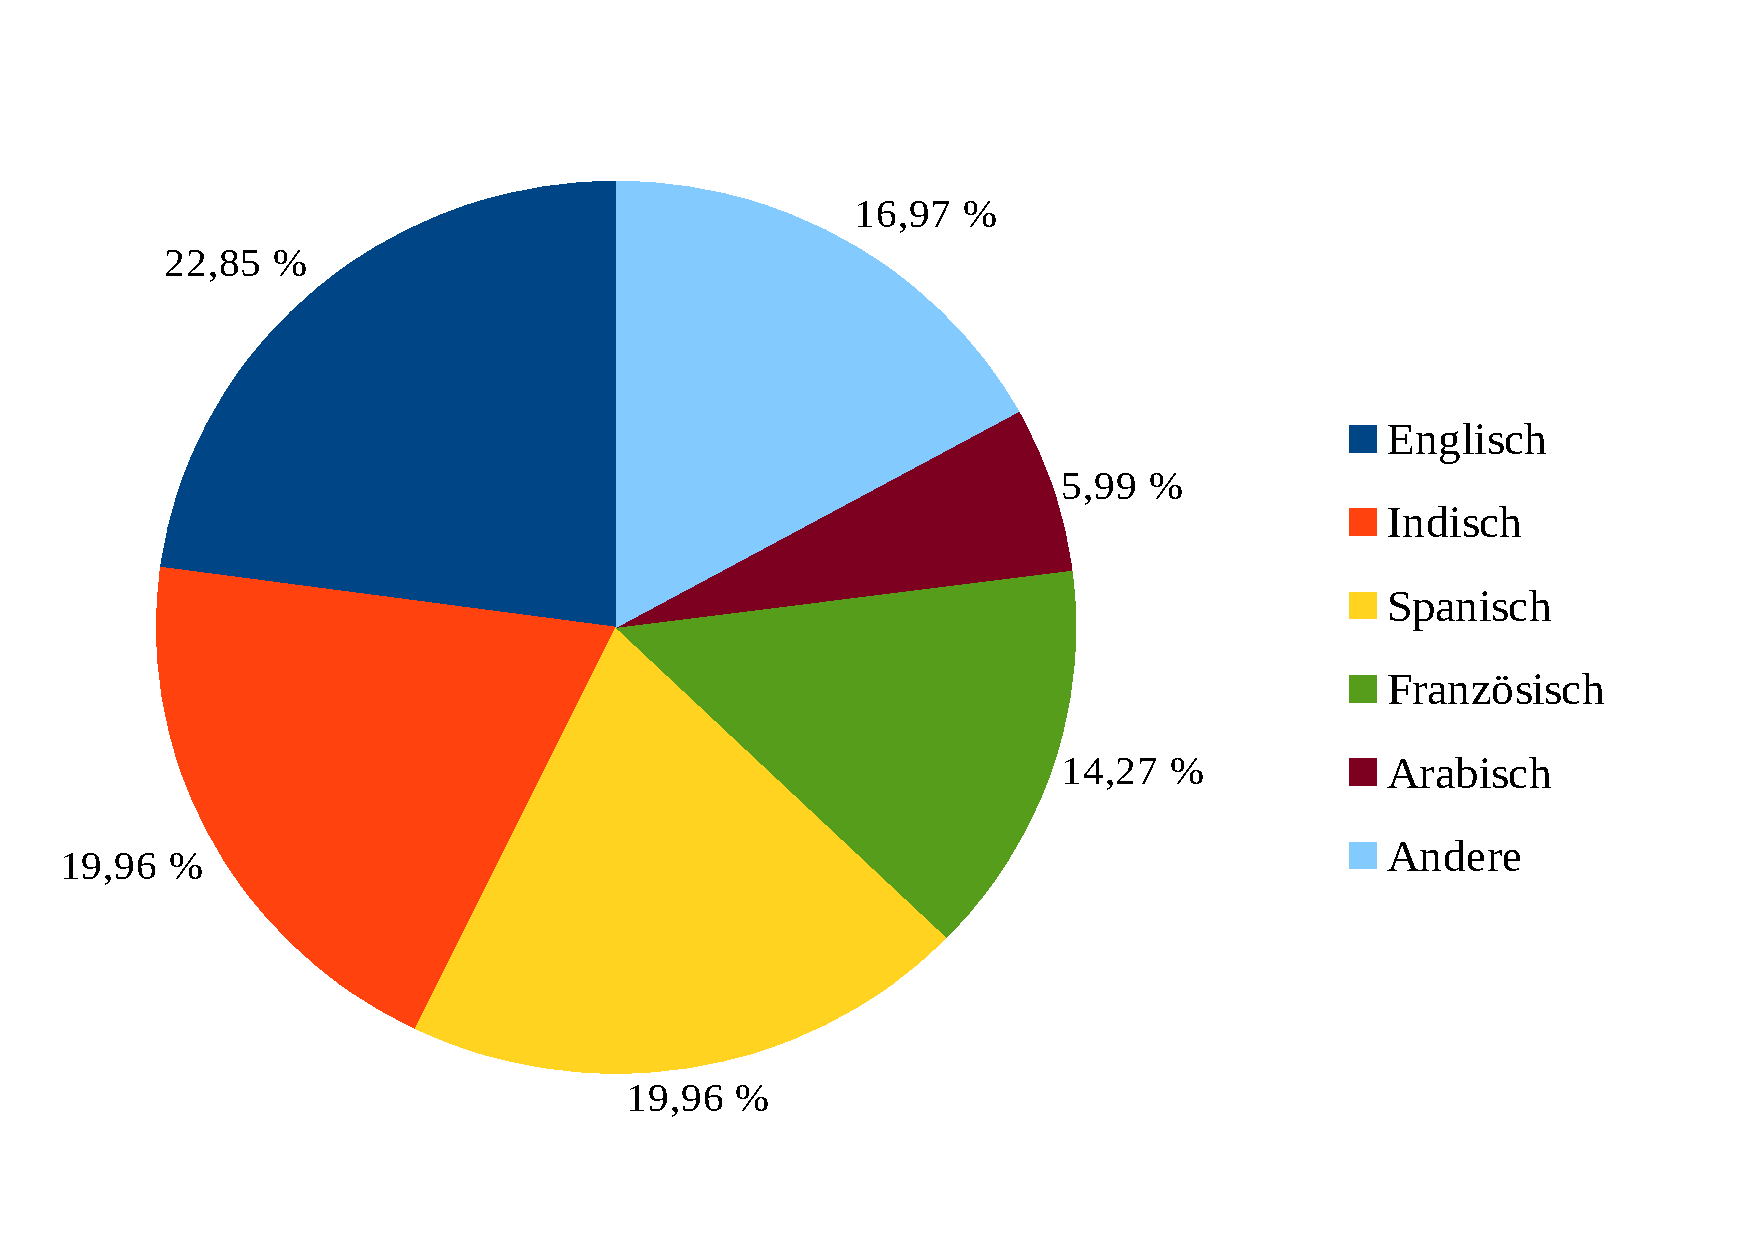
\includegraphics[width=12cm]{Bilder/Umfrage/Umfrage_Sprachen.pdf}
		\caption{Umfragewerte zu gewünschten Spracherweiterungen\label{fig:umfrage_sprachen_diagram}\protect\footnotemark}
	\end{center}
\end{figure}

\subsubsection{Einfachere Stundenplanerstellung}


\footnotetext{Brysiuk, Lehmann (2019)} %auf richtiger Seite wie grafik???

Aus den Gesprächen mit dem International Office der Hochschule Hof hat sich ergeben, dass viele Internationale Studierende große Probleme damit haben, einen vollständigen Stundenplan über eine der \acp{App} zu pflegen. Das liegt vor allem daran, dass viele der Internationals Vorlesungen aus verschiedenen Studiengängen und teilweise sogar aus verschiedenen Fakultäten belegen. Es ist zwar prinzipiell möglich, einen solchen Stundenplan in den \acp{App} zu erstellen, allerdings ist dies nicht einmal vorgesehen und funktioniert so nur durch Zufall. Die internationalen Studierenden, die sich bei der Bedienung der Anwendungen ohnehin schon schwer tun, finden solche Schlupflöcher einfach nicht und befinden die \acp{App} somit als unbrauchbar. Das International Office wünscht sich deshalb, das die personalisierte Stundenplanzusammenstellung in den Anwendungen oder in einer neuen Anwendung deutlich flexibler wird.  

\section{Sprachenzentrum\label{sec:anforderungen_sz}}

Die Hochschule Hof bietet neben ihren regulären Veranstaltungen, die durch die Fakultäten organisiert und gehalten werden, ebenfalls eine reiche Auswahl an Sprachkursen an. Diese werden vom Sprachenzentrum der Hochschule Hof veranstaltet. Die hohe Bedeutung von gut organisierten Sprachkursen an einer akademischen Institution ist unbestreitbar. Das Sprachenzentrum selbst formuliert es wie folgt:
\begin{quote}
Sprachen sind das Tor zur Welt; unerlässlich in einer akademischen Karriere. Daher wird an der Hochschule Hof als international ausgerichteter Hochschule besonderer Wert auf eine profunde Sprachausbildung gelegt.
\autocite[][]{szweb}
\end{quote}
Konkret werden aktuell an der Hochschule Hof allgemeine Sprachkurse in den Sprachen Englisch, Spanisch, Französisch, Chinesisch, Russisch, Türkisch sowie Deutsch angeboten. Diese werden im Rahmen von Pflicht- und Wahlveranstaltungen für Studierende, sowie als \ac{UNIcert}-Prüfungen und \ac{TestDaF} angeboten.
\\
\linebreak
Jedoch bringt das Angebot von zusätzlichen Veranstaltungen, die nicht von den Fakultäten organisiert werden, einige Herausforderungen mit sich. Diese werden im folgenden aufgelistet, wobei mögliche Lösungen im Rahmen dieser Bachelorarbeit erörtert werden.

\subsection{Problem\label{sec:prob_sz}}

Das Ziel der Hochschule Hof ist es, den Studierenden einen einfachen und übersichtlichen Zugang zu den benötigten Informationen des Sprachenzentrums zu geben. Vor allem bei den internationalen Besuchern der Vorlesungen ist es wichtig, dass sie das Angebot der Sprachkurse leicht einsehen können, denn für sie sind deutsche Sprachkurse oft verpflichtend. Aber auch reguläre Studierende belegen oft Sprachkurse, entweder, um ihre Kenntnisse aus vorangegangenen Kursen zu vertiefen oder um sich neue Sprachen anzueignen. So geben etwa 89\% der deutschsprachigen Studenten an, dass sie Informationen zum Sprachenzentrum gerne mit in eine allgemeine Hochschulanwendung eingebunden hätten. Auffällig ist hier auch die Statistik bei den nicht deutschsprachigen Studierenden. Hier sind es bereits 93\%, die eine Erweiterung der aktuellen Anwendungen mit dem Angebot an Sprachkursen begrüßen würden. Hier hilft oft auch die Nutzung der Website nicht weiter. Somit sind zum Aufrufen allgemeiner Infos des Sprachzentrums bereits fünf Klicks von der Startseite aus gezählt nötig, für Änderungen im Kursprogramm sind es sogar schon sechs\autocite[][]{umfrage}.
\\
\linebreak
Für die internationalen Studierenden ist hier die Informationssuche deutlich schwieriger, da diese Informationen im englischen Angebot des Sprachenzentrums auf der Hochschul Website nicht aufgeführt werden. Zudem ist die Informationsbeschaffung der Studenten in Bezug auf die Sprachkursinformationen im Vergleich zu den fachbezogenen Vorlesungen deutlich unterscheidbar. In der Android \ac{App} ist das Sprachenzentrum beispielsweise als eigener Studiengang geführt und kann nur so in den Stundenplan aufgenommen werden. Dies kann bei vielen Studierenden zu Verwirrung führen. Andere Nutzer kennen diesen Spezialfall in der Implementierung der Anwendung nicht und können die Stunden ihrer Sprachkurse somit auch nicht in ihren persönlichen Stundenplan aufnehmen. Zudem sind Sprachkursinformationen, sowohl allgemeine Informationen als auch Stundenpläne zu dem Kursangebot, auf der Website der Hochschule separat geführt. Somit ist die Suche nach den Sprachkursen, die ein Studierender nutzen möchte, mit einem deutlichen Mehraufwand gegenüber der regulären Vorlesungssuche verbunden. 

\subsection{Funktionale Anforderungen\label{sec:anf_sz}}

Aus den oben genannten Problemen der aktuellen Informationsdarstellung ergeben sich einige Anforderungen an eine neue Hochschul-\ac{App}, welche nun weiter erörtert werden.

\subsubsection{Einbinden von Sprachkursinformationen}

Eine Anforderung des Sprachenzentrums ist es, die Informationen, die es anbietet, in eine Hochschul-\ac{App} einzubinden. Der Fokus sollte darauf liegen, das Sprachangebot der Hochschule wie normale Vorlesungen zu behandeln, zu denen die Studierenden ebenfalls alle relevanten Informationen abgreifen können.

\subsubsection{Mehrsprachige Sprachkursinformationen}

Des weiteren ist es wünschenswert, die Informationen des Sprachenzentrums nicht nur in deutscher Sprache, sondern auch in Fremdsprachen, vor allem in Englisch, einzubinden. Dabei sollte der Fokus nicht nur auf allgemeinen Informationen liegen, sondern auf spezielleren Daten, wie Details zu Stundenplanänderungen im Bereich der Sprachkurse. 

\subsubsection{Einheitliche Darstellung}

Es ist wünschenswert, dass die Sprachkurse im selben Rahmen wie die regulären, verpflichtenden Vorlesungen der Studierenden dargestellt werden. Es sollte also möglich sein, die belegten Sprachkurse genauso leicht in einen personalisierten Stundenplan zu übernehmen, wie die regulär belegten Vorlesungen. 

\subsubsection{Vollständige Informationsdarstellung}

Zu den Sprachkursen sollten nicht nur allgemeine Informationen wie Veranstaltungsort und Zeitpunkt stehen, stattdessen fordert das Sprachenzentrum die genauere Einbindung einiger Details. Eines dieser Details sind die Sprachniveaus der angebotenen Kurse. Werden diese angezeigt, ist es auch wichtig, dass ersichtlich ist, ob ein Kurs einen sogenannten Placementtest benötigt, der die Studierenden zur Teilnahme am Kurs berechtigt.
 
\subsubsection{Vorgeschlagene Features}

Das Sprachenzentrum hat des weiteren einige Vorschläge zur Verbesserung der Nutzbarkeit einer neuen Anwendung erbracht. 
%1
Einer dieser Ideen ist die Möglichkeit, bei der Auswahl eines Sprachkurses in einen personalisierten Stundenplan direkt zu der Anmeldung dieses Kurses weitergeleitet zu werden.
%2
Zudem kann es hilfreich sein, angebotene Sprachkurse nach deren Niveau filtern zu können.
%3
Ebenso kann eine verbesserte Hochschul-\ac{App} dem Nutzer auch die angebotenen Sprachkurse anzeigen, die in den freien Stunden seines personalisierten Stundenplans angeboten werden. So kann er die Freizeit zwischen seinen Pflichtveranstaltungen sinnvoll nutzen und die Sprachkurse werden optimal ausgelastet.

\section{Pflichtenheft\label{sec:pfilchtenheft}}

Die in Kapitel \ref{sec:anforderung} gesammelten Anforderungen können für das Projekt der neuen Hoch\-schul-\ac{App} als Lastenheft angesehen werden. Dieses wird benötigt, um klar definieren zu können, was der Auftraggeber und andere Interessenparteien von einem Projekt erwarten. Was ein Lastenheft jedoch nicht definiert ist der Rahmen und Umfang der Anforderungen, die auch im späteren Implementierungsprozess umgesetzt werden. Dafür muss vor der Implementierung noch ein Pflichtenheft definiert werden. Die darin definierten Pflichten sind dann genau die Anforderungen, die im Rahmen der zu dieser Bachelorarbeit parallel geführten Praxisarbeit umgesetzt werden\autocite[Vgl.][]{dnpa}. Um das Lastenheft und das Pflichtenheft klar voneinander trennen zu können wird das Pflichtenheft in der eben genannten Praxisarbeit definiert. Eine Gegenüberstellung der geplanten und umgesetzten Anforderungen kann dann anhand der Referenznummern  aus dem Lastenheft erfolgen. Das Lastenheft kann dem Anhang dieser Arbeit entnommen werden.
